% Options for packages loaded elsewhere
\PassOptionsToPackage{unicode}{hyperref}
\PassOptionsToPackage{hyphens}{url}
%
\documentclass[
  english,
  man,mask]{apa6}
\usepackage{amsmath,amssymb}
\usepackage{lmodern}
\usepackage{ifxetex,ifluatex}
\ifnum 0\ifxetex 1\fi\ifluatex 1\fi=0 % if pdftex
  \usepackage[T1]{fontenc}
  \usepackage[utf8]{inputenc}
  \usepackage{textcomp} % provide euro and other symbols
\else % if luatex or xetex
  \usepackage{unicode-math}
  \defaultfontfeatures{Scale=MatchLowercase}
  \defaultfontfeatures[\rmfamily]{Ligatures=TeX,Scale=1}
\fi
% Use upquote if available, for straight quotes in verbatim environments
\IfFileExists{upquote.sty}{\usepackage{upquote}}{}
\IfFileExists{microtype.sty}{% use microtype if available
  \usepackage[]{microtype}
  \UseMicrotypeSet[protrusion]{basicmath} % disable protrusion for tt fonts
}{}
\makeatletter
\@ifundefined{KOMAClassName}{% if non-KOMA class
  \IfFileExists{parskip.sty}{%
    \usepackage{parskip}
  }{% else
    \setlength{\parindent}{0pt}
    \setlength{\parskip}{6pt plus 2pt minus 1pt}}
}{% if KOMA class
  \KOMAoptions{parskip=half}}
\makeatother
\usepackage{xcolor}
\IfFileExists{xurl.sty}{\usepackage{xurl}}{} % add URL line breaks if available
\IfFileExists{bookmark.sty}{\usepackage{bookmark}}{\usepackage{hyperref}}
\hypersetup{
  pdftitle={Reminder about Confidence Intervals},
  pdfauthor={Marie Delacre1, Daniel Lakens2, Christophe Ley3, Limin Liu3, \& Christophe Leys1},
  pdflang={en-EN},
  hidelinks,
  pdfcreator={LaTeX via pandoc}}
\urlstyle{same} % disable monospaced font for URLs
\usepackage{graphicx}
\makeatletter
\def\maxwidth{\ifdim\Gin@nat@width>\linewidth\linewidth\else\Gin@nat@width\fi}
\def\maxheight{\ifdim\Gin@nat@height>\textheight\textheight\else\Gin@nat@height\fi}
\makeatother
% Scale images if necessary, so that they will not overflow the page
% margins by default, and it is still possible to overwrite the defaults
% using explicit options in \includegraphics[width, height, ...]{}
\setkeys{Gin}{width=\maxwidth,height=\maxheight,keepaspectratio}
% Set default figure placement to htbp
\makeatletter
\def\fps@figure{htbp}
\makeatother
\setlength{\emergencystretch}{3em} % prevent overfull lines
\providecommand{\tightlist}{%
  \setlength{\itemsep}{0pt}\setlength{\parskip}{0pt}}
\setcounter{secnumdepth}{-\maxdimen} % remove section numbering
% Make \paragraph and \subparagraph free-standing
\ifx\paragraph\undefined\else
  \let\oldparagraph\paragraph
  \renewcommand{\paragraph}[1]{\oldparagraph{#1}\mbox{}}
\fi
\ifx\subparagraph\undefined\else
  \let\oldsubparagraph\subparagraph
  \renewcommand{\subparagraph}[1]{\oldsubparagraph{#1}\mbox{}}
\fi
% Manuscript styling
\usepackage{upgreek}
\captionsetup{font=singlespacing,justification=justified}

% Table formatting
\usepackage{longtable}
\usepackage{lscape}
% \usepackage[counterclockwise]{rotating}   % Landscape page setup for large tables
\usepackage{multirow}		% Table styling
\usepackage{tabularx}		% Control Column width
\usepackage[flushleft]{threeparttable}	% Allows for three part tables with a specified notes section
\usepackage{threeparttablex}            % Lets threeparttable work with longtable

% Create new environments so endfloat can handle them
% \newenvironment{ltable}
%   {\begin{landscape}\centering\begin{threeparttable}}
%   {\end{threeparttable}\end{landscape}}
\newenvironment{lltable}{\begin{landscape}\centering\begin{ThreePartTable}}{\end{ThreePartTable}\end{landscape}}

% Enables adjusting longtable caption width to table width
% Solution found at http://golatex.de/longtable-mit-caption-so-breit-wie-die-tabelle-t15767.html
\makeatletter
\newcommand\LastLTentrywidth{1em}
\newlength\longtablewidth
\setlength{\longtablewidth}{1in}
\newcommand{\getlongtablewidth}{\begingroup \ifcsname LT@\roman{LT@tables}\endcsname \global\longtablewidth=0pt \renewcommand{\LT@entry}[2]{\global\advance\longtablewidth by ##2\relax\gdef\LastLTentrywidth{##2}}\@nameuse{LT@\roman{LT@tables}} \fi \endgroup}

% \setlength{\parindent}{0.5in}
% \setlength{\parskip}{0pt plus 0pt minus 0pt}

% \usepackage{etoolbox}
\makeatletter
\patchcmd{\HyOrg@maketitle}
  {\section{\normalfont\normalsize\abstractname}}
  {\section*{\normalfont\normalsize\abstractname}}
  {}{\typeout{Failed to patch abstract.}}
\patchcmd{\HyOrg@maketitle}
  {\section{\protect\normalfont{\@title}}}
  {\section*{\protect\normalfont{\@title}}}
  {}{\typeout{Failed to patch title.}}
\makeatother
\shorttitle{CI REMINDER}
\keywords{\newline\indent Word count: 273}
\DeclareDelayedFloatFlavor{ThreePartTable}{table}
\DeclareDelayedFloatFlavor{lltable}{table}
\DeclareDelayedFloatFlavor*{longtable}{table}
\makeatletter
\renewcommand{\efloat@iwrite}[1]{\immediate\expandafter\protected@write\csname efloat@post#1\endcsname{}}
\makeatother
\usepackage{lineno}

\linenumbers
\usepackage{csquotes}
\ifxetex
  % Load polyglossia as late as possible: uses bidi with RTL langages (e.g. Hebrew, Arabic)
  \usepackage{polyglossia}
  \setmainlanguage[]{english}
\else
  \usepackage[main=english]{babel}
% get rid of language-specific shorthands (see #6817):
\let\LanguageShortHands\languageshorthands
\def\languageshorthands#1{}
\fi
\ifluatex
  \usepackage{selnolig}  % disable illegal ligatures
\fi
\newlength{\cslhangindent}
\setlength{\cslhangindent}{1.5em}
\newlength{\csllabelwidth}
\setlength{\csllabelwidth}{3em}
\newenvironment{CSLReferences}[2] % #1 hanging-ident, #2 entry spacing
 {% don't indent paragraphs
  \setlength{\parindent}{0pt}
  % turn on hanging indent if param 1 is 1
  \ifodd #1 \everypar{\setlength{\hangindent}{\cslhangindent}}\ignorespaces\fi
  % set entry spacing
  \ifnum #2 > 0
  \setlength{\parskip}{#2\baselineskip}
  \fi
 }%
 {}
\usepackage{calc}
\newcommand{\CSLBlock}[1]{#1\hfill\break}
\newcommand{\CSLLeftMargin}[1]{\parbox[t]{\csllabelwidth}{#1}}
\newcommand{\CSLRightInline}[1]{\parbox[t]{\linewidth - \csllabelwidth}{#1}\break}
\newcommand{\CSLIndent}[1]{\hspace{\cslhangindent}#1}

\title{Reminder about Confidence Intervals}
\author{Marie Delacre\textsuperscript{1}, Daniel Lakens\textsuperscript{2}, Christophe Ley\textsuperscript{3}, Limin Liu\textsuperscript{3}, \& Christophe Leys\textsuperscript{1}}
\date{}


\authornote{

Correspondence concerning this article should be addressed to Marie Delacre, CP191, avenue F.D. Roosevelt 50, 1050 Bruxelles. E-mail: \href{mailto:marie.delacre@ulb.be}{\nolinkurl{marie.delacre@ulb.be}}

}

\affiliation{\vspace{0.5cm}\textsuperscript{1} Université Libre de Bruxelles, Service of Analysis of the Data (SAD), Bruxelles, Belgium\\\textsuperscript{2} Eindhoven University of Technology, Human Technology Interaction Group, Eindhoven, the Netherlands\\\textsuperscript{3} Universiteit Gent, Department of Applied Mathematics, Computer Science and Statistics, Gent, Belgium}

\begin{document}
\maketitle

\hypertarget{how-to-compute-a-confidence-interval-around-a-point-estimator}{%
\subsubsection{How to compute a confidence interval around a point estimator}\label{how-to-compute-a-confidence-interval-around-a-point-estimator}}

As illustration, we will explain how to compute a confidence interval around Cohen's \(d\) (the explanation would be very similar for all other estimators). Under the assumption of iid normal distribution of residuals with equal population variances across groups, in order to test the null hypothesis that \(\mu_1-\mu_2= (\mu_1-\mu_2)_0\), we can compute the following quantity:
\begin{equation*} 
t_{Student}=\frac{(\bar{X_1}-\bar{X_2})-(\mu_1-\mu_2)_0}{SE}
\label{eq:tstudent}
\end{equation*}
with \(SE = S_{pooled} \times \sqrt{\frac{1}{n_1}+\frac{1}{n_2}}\), \(S_{pooled} = \sqrt{\frac{(n_1-1) \times S^2_1+(n_2-1)\times S^2_2}{n_1+n_2-2}}\) and \(S_j\) = the standard deviation of the \(j^{th}\) sample (\(j=1,2\)). Under the null hypothesis, this quantity will follow a central \emph{t}-distribution with \(n_1+n_2-2\) degrees of freedom. However, when the null hypothesis is false, the distribution of this quantity is not centered and a noncentral \emph{t}-distribution arises (Cumming \& Finch, 2001), as illustrated in Figure \ref{fig:SAMPLMEANDIFF3}. Noncentral \emph{t}-distributions are described by two parameters: degrees of freedom (\(df\)) and noncentrality parameter (that we will call \(\Delta\), Cumming \& Finch, 2001), the last being a function of the population effect size (\(\delta\)) and sample sizes (\(n_1\) and \(n_2\)):
\begin{equation*}
\Delta = \frac{\delta}{\sqrt{\frac{1}{n_1}+\frac{1}{n_2}}}
\label{eq:ncp}
\end{equation*}
with \(\delta=\frac{(\mu_1-\mu_2)-(\mu_1-\mu_2)_0}{\sigma_{pooled}}\), \(\sigma_{pooled} = \sqrt{\frac{(n_1-1) \times \sigma^2_1+(n_2-1)\times \sigma^2_2}{n_1+n_2-2}}\) and \(\sigma_j\) = the standard deviation of the \(j^{th}\) population (\(j=1,2\)). Considering the link between \(\Delta\) and \(\delta\), it is possible to compute confidence limits for \(\Delta\) and multiply them by \(\sqrt{\frac{1}{n_1}+\frac{1}{n_2}}\) in order to have confidence limits for \(\delta\). In other words, we first need to determine the noncentrality parameters of the \emph{t}-distributions for which \(t_{Student}\) corresponds respectively to the quantiles \(\left(1-\frac{\alpha}{2}\right)\) and \(\frac{\alpha}{2}\):
\[P[t_{df, \Delta_L} \geq t_{Student}] = \frac{\alpha}{2} \]
\[P[t_{df, \Delta_U} \leq t_{Student}] = \frac{\alpha}{2} \]
with \(df = n_1+n_2-2\). Second, we multiply \(\Delta_L\) and \(\Delta_U\) by \(\sqrt{\frac{1}{n_1}+\frac{1}{n_2}}\) in order to define \(\delta_L\) and \(\delta_U\):
\[\delta_L = \Delta_L \times \sqrt{\frac{1}{n_1}+\frac{1}{n_2}}\]
\[\delta_U = \Delta_U \times \sqrt{\frac{1}{n_1}+\frac{1}{n_2}}\]

\begin{figure}
\centering
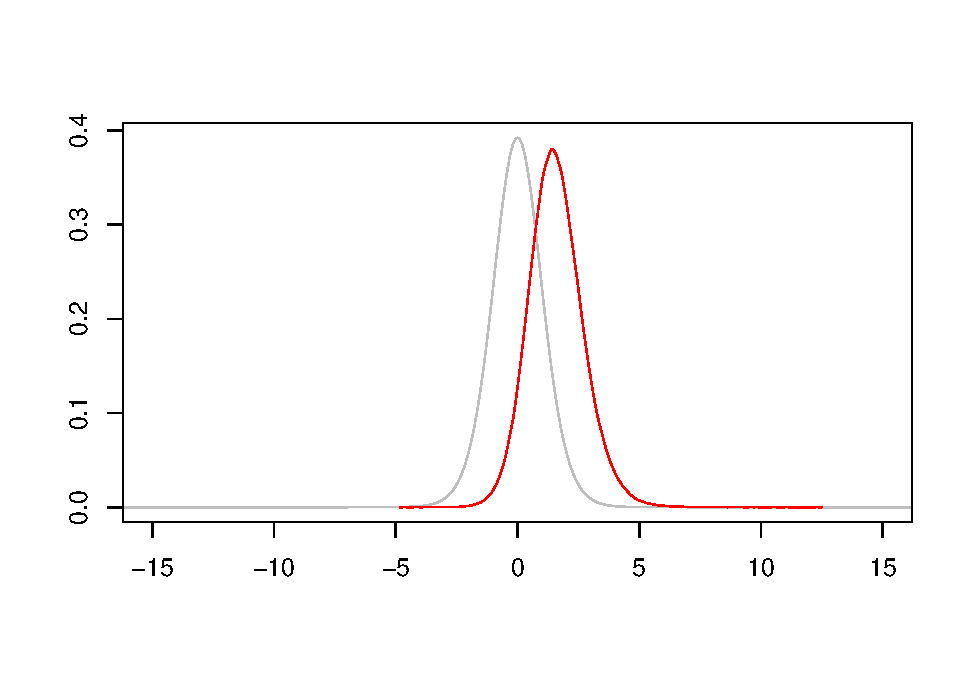
\includegraphics{CI_files/figure-latex/SAMPLMEANDIFF3-1.pdf}
\caption{\label{fig:SAMPLMEANDIFF3}Sampling distribution of \(t=\frac{(\bar{X_1}-\bar{X_2})-(\mu_1-\mu_2)_0}{SE}\) when the null hypothesis is true (in grey) and when the null hypothesis is false, with \((\mu_1-\mu_2)-(\mu_1-\mu_2)_0=4\) and \(SE=5\) (in red).}
\end{figure}

\hypertarget{reference}{%
\section*{Reference}\label{reference}}
\addcontentsline{toc}{section}{Reference}

\hypertarget{refs}{}
\begin{CSLReferences}{1}{0}
\leavevmode\hypertarget{ref-Cumming_Finch_2001}{}%
Cumming, G., \& Finch, S. (2001). A primer on the understanding, use, and calculation of confidence intervals that are based on central and noncentral distributions. \emph{{E}ducational and {P}sychological {M}easurement}, \emph{61}(4), 532--574.

\end{CSLReferences}


\end{document}
